\documentclass[12pt,a4paper]{article}

% --- GÓI HỖ TRỢ TIẾNG VIỆT VÀ FONT ---
\usepackage[utf8]{inputenc}
\usepackage[vietnamese]{babel}
\usepackage{times}
\usepackage{graphicx}
\graphicspath{{figures/}}

% --- CĂN CHỈNH LỀ VÀ KHOẢNG CÁCH ---
\usepackage[left=2.5cm, right=2cm, top=2.5cm, bottom=2.5cm]{geometry}
\usepackage{indentfirst}
\usepackage{setspace}
\setstretch{1.2}
\usepackage{mdframed}
\usepackage{amsmath}
\usepackage{amssymb}
\usepackage{float}
\usepackage{array}
\usepackage{booktabs}
\usepackage{xcolor}
\usepackage{listings}

% Định nghĩa bảng màu code
\definecolor{codegreen}{rgb}{0.13, 0.55, 0.13}    % Màu chú thích (comment)
\definecolor{codepurple}{rgb}{0.58, 0, 0.82}      % Màu chuỗi ký tự (string)
\definecolor{codeblue}{rgb}{0.0, 0.2, 0.8}        % Màu từ khóa (keywords)
\definecolor{backcolour}{rgb}{0.97, 0.97, 0.97}   % Màu nền nhẹ
\definecolor{linegray}{rgb}{0.5, 0.5, 0.5}        % Màu số dòng

\lstdefinestyle{scilabstyle}{
    backgroundcolor=\color{backcolour},
    commentstyle=\color{codegreen}\itshape,
    keywordstyle=\color{codeblue}\bfseries,
    numberstyle=\tiny\color{linegray},
    stringstyle=\color{codepurple},
    basicstyle=\ttfamily\footnotesize,
    breakatwhitespace=false,
    breaklines=true,
    breakindent=15pt,
    postbreak=\mbox{\textcolor{linegray}{$\hookrightarrow$}\space},
    captionpos=b,
    keepspaces=true,
    numbers=left,
    numbersep=8pt,
    showspaces=false,
    showstringspaces=false,
    showtabs=false,
    tabsize=2,
    frame=single,
    rulecolor=\color{black!15},
    xleftmargin=1.5em,
    framexleftmargin=1.5em
}

% Khung kết quả console Scilab
\lstdefinestyle{consolestyle}{
    backgroundcolor=\color{white},
    basicstyle=\ttfamily\footnotesize,
    frame=single,
    rulecolor=\color{black!40},
    numbers=none,
    keepspaces=true,
    showstringspaces=false,
    xleftmargin=3em,
    xrightmargin=3em,
    title={\footnotesize\textsf{Scilab 2026.1.0 Console}}
}

% Khung đề bài dùng chung cho các bài tập
\mdfdefinestyle{exbox}{
    linewidth=0.8pt,
    linecolor=black,
    backgroundcolor=white,
    innertopmargin=10pt,
    innerbottommargin=10pt,
    innerleftmargin=12pt,
    innerrightmargin=12pt,
    skipabove=10pt,
    skipbelow=10pt
}

% --- GÓI HỖ TRỢ ĐƯỜNG DẪN VÀ THAM KHẢO ---
\usepackage{hyperref}
\hypersetup{
    colorlinks=true,
    linkcolor=black,
    urlcolor=blue,
    citecolor=black
}

% Ký hiệu cặp biến đổi Fourier
\newcommand{\fpair}{\overset{\mathcal{F}}{\longleftrightarrow}}

% --- THIẾT KẾ PHẦN TIÊU ĐỀ BÁO CÁO ---
\title{
    \vspace{-1.5cm}
    \large\textbf{Xử Lý Tín Hiệu Số} \\
    \normalsize HK261 \quad -- \quad CO2036 \\[1em]
    \Large\textbf{BÀI THỰC HÀNH 6 XỬ LÝ TÍN HIỆU SỐ}
}

\author{
    \textbf{Trần Minh Quang} -- \textbf{2412855}
}

\date{19/11/2026}

\begin{document}

\maketitle

% --- PHẦN TỔNG QUAN ---
\begin{abstract}
\noindent\textbf{Tổng Quan:} Bài thực hành 6 tìm biến đổi Fourier của các tín hiệu liên tục và rời rạc, sau đó dùng Scilab vẽ phổ biên độ và phổ pha của tín hiệu và của hệ LTI. Kết quả tính số trên Scilab trùng với các công thức giải tích, sai lệch chỉ ở mức sai số làm tròn của máy tính.
\end{abstract}

\vspace{0.5cm}

% --- NỘI DUNG CHÍNH ---
\section{Giới Thiệu}
Các lab trước phân tích tín hiệu và hệ thống trong miền thời gian và miền $z$. Lab này chuyển sang miền tần số: biến đổi Fourier cho biết tín hiệu gồm những thành phần tần số nào (phổ biên độ) và mỗi thành phần bị dịch pha bao nhiêu (phổ pha). Với tín hiệu rời rạc, biến đổi Fourier $X(\omega)$ chính là biến đổi Z tính trên đường tròn đơn vị $z = e^{j\omega}$, và luôn tuần hoàn với chu kỳ $2\pi$, nên chỉ cần vẽ phổ trong đoạn $[-\pi, \pi]$. Công cụ sử dụng là Scilab 2026.1.0.

\section{Mục Tiêu}
\begin{itemize}
    \item Tìm biến đổi Fourier của tín hiệu liên tục và tín hiệu rời rạc theo định nghĩa và theo các tính chất.
    \item Tìm đáp ứng tần số $H(\omega)$ của hệ LTI từ phương trình sai phân, và tìm ngõ ra bằng tính chất $Y(\omega) = H(\omega)X(\omega)$.
    \item Dùng Scilab vẽ phổ biên độ $|X(\omega)|$ và phổ pha $\angle X(\omega)$.
\end{itemize}

\section{Phương Pháp}
\begin{itemize}
    \item \textbf{Bài 1--2:} tính trực tiếp từ định nghĩa
    \[
        X(\Omega) = \int_{-\infty}^{\infty} x(t) e^{-j\Omega t}\, dt,
        \qquad
        X(\omega) = \sum_{n=-\infty}^{\infty} x(n) e^{-j\omega n},
    \]
    dùng tổng cấp số nhân và các tính chất dịch thời gian, đối ngẫu.
    \item \textbf{Bài 3--5:} tìm công thức $X(\omega)$ hoặc $H(\omega)$, sau đó viết script Scilab tính phổ trên lưới 1001 điểm tần số trong $[-\pi, \pi]$ và vẽ phổ biên độ, phổ pha. Hàm \texttt{dtft} tự viết tính trực tiếp tổng $\sum x(n) e^{-j\omega n}$ dưới dạng phép nhân ma trận, dùng để đối chiếu với công thức giải tích. Pha được tính bằng \texttt{atan(imag(X), real(X))}, cho giá trị trong $(-\pi, \pi]$.
    \item \textbf{Kiểm chứng:} mọi công thức của Bài 1--2 đều được em so với tổng (hoặc tích phân) tính số tại nhiều giá trị tần số; sai lệch đều xấp xỉ 0.
\end{itemize}

\section{Nội Dung Thực Hành}

% =====================================================================
\subsection{Bài tập 1 -- Biến đổi Fourier của tín hiệu liên tục}
\begin{mdframed}[style=exbox]
\noindent\textbf{Bài tập 1.} Tìm biến đổi Fourier của các tín hiệu:
\[
    x_1(t) =
    \begin{cases}
        1 - \dfrac{|t|}{\tau}, & |t| \le \tau \\[1ex]
        0, & |t| > \tau
    \end{cases}
    \qquad\qquad
    x_2(t) = e^{j\omega_0 t}.
\]
\end{mdframed}

\textbf{$x_1(t)$ -- xung tam giác.} Vì $x_1(t)$ là hàm chẵn nên phần ảo của tích phân triệt tiêu:
\[
    X_1(\Omega) = \int_{-\tau}^{\tau} \left(1 - \frac{|t|}{\tau}\right) e^{-j\Omega t}\, dt
    = 2\int_{0}^{\tau} \left(1 - \frac{t}{\tau}\right) \cos(\Omega t)\, dt.
\]
Tích phân từng phần:
\[
    2\int_{0}^{\tau} \left(1 - \frac{t}{\tau}\right) \cos(\Omega t)\, dt
    = 2\left[\left(1 - \frac{t}{\tau}\right)\frac{\sin\Omega t}{\Omega}\right]_0^{\tau} + \frac{2}{\tau\Omega}\int_0^{\tau} \sin(\Omega t)\, dt
    = \frac{2\left(1 - \cos\Omega\tau\right)}{\tau\Omega^2}.
\]
Dùng $1 - \cos\Omega\tau = 2\sin^2\frac{\Omega\tau}{2}$:
\begin{equation}
    X_1(\Omega) = \frac{4\sin^2\left(\frac{\Omega\tau}{2}\right)}{\tau\Omega^2} = \tau \left[\frac{\sin\left(\Omega\tau/2\right)}{\Omega\tau/2}\right]^2.
\end{equation}
Phổ là hàm thực, không âm, có giá trị lớn nhất $X_1(0) = \tau$ (bằng diện tích tam giác) và bằng 0 tại $\Omega = \frac{2\pi k}{\tau}$, $k \ne 0$. Có thể hiểu kết quả này theo cách khác: xung tam giác là tích chập của hai xung chữ nhật độ rộng $\tau$, nên phổ của nó tỉ lệ với bình phương hàm sinc.

\textbf{$x_2(t)$ -- hàm mũ phức.} $x_2(t)$ không khả tích tuyệt đối nên biến đổi Fourier chỉ tồn tại theo nghĩa hàm suy rộng. Xét $X_2(\Omega) = 2\pi\delta(\Omega - \omega_0)$; biến đổi ngược của nó là
\[
    \frac{1}{2\pi}\int_{-\infty}^{\infty} 2\pi\delta(\Omega - \omega_0)\, e^{j\Omega t}\, d\Omega = e^{j\omega_0 t}.
\]
Do đó
\begin{equation}
    X_2(\Omega) = 2\pi\,\delta(\Omega - \omega_0).
\end{equation}
Tín hiệu chỉ chứa đúng một tần số $\omega_0$ nên phổ là một xung Dirac duy nhất tại $\Omega = \omega_0$.

\textbf{Kiểm tra:} tính tích phân số cho $X_1(\Omega)$ với $\tau = 1.5$ tại $\Omega = 0.5, 2, 5$ được $1.430993$, $0.663331$, $0.034846$, trùng với công thức.

% =====================================================================
\subsection{Bài tập 2 -- Biến đổi Fourier của tín hiệu rời rạc}
\begin{mdframed}[style=exbox]
\noindent\textbf{Bài tập 2.} Tìm biến đổi Fourier của các tín hiệu:
\begin{itemize}
    \item $x_1(n) = u(n) - u(n-6)$, \qquad $x_2(n) = 2^n u(-n)$
    \item[a.] $x_3(n) = \left(\frac{1}{4}\right)^n u(n+4)$
    \item[b.] $x_4(n) = 2 - \frac{1}{2}n$ khi $|n| \le 4$, \quad $x_4(n) = 0$ khi $|n| > 4$
    \item[c.] $x_5(n) = |a|^n \sin(\omega_0 n)$, \quad $|a| < 1$
\end{itemize}
\end{mdframed}

\textbf{$x_1(n) = u(n) - u(n-6)$:} xung chữ nhật gồm 6 mẫu bằng 1 tại $n = 0, \dots, 5$. Dùng tổng cấp số nhân:
\[
    X_1(\omega) = \sum_{n=0}^{5} e^{-j\omega n} = \frac{1 - e^{-j6\omega}}{1 - e^{-j\omega}}
    = \frac{e^{-j3\omega}\left(e^{j3\omega} - e^{-j3\omega}\right)}{e^{-j\omega/2}\left(e^{j\omega/2} - e^{-j\omega/2}\right)}
\]
\begin{equation}
    X_1(\omega) = e^{-j5\omega/2}\, \frac{\sin(3\omega)}{\sin(\omega/2)}.
\end{equation}

\textbf{$x_2(n) = 2^n u(-n)$:} tín hiệu chỉ khác 0 khi $n \le 0$. Đặt $m = -n$:
\begin{equation}
    X_2(\omega) = \sum_{n=-\infty}^{0} 2^n e^{-j\omega n} = \sum_{m=0}^{\infty} \left(\tfrac{1}{2}e^{j\omega}\right)^m = \frac{1}{1 - \frac{1}{2}e^{j\omega}}.
\end{equation}
Chuỗi hội tụ vì $\left|\frac{1}{2}e^{j\omega}\right| = \frac{1}{2} < 1$.

\textbf{a. $x_3(n) = \left(\frac{1}{4}\right)^n u(n+4)$:} tín hiệu bắt đầu từ $n = -4$:
\begin{equation}
    X_3(\omega) = \sum_{n=-4}^{\infty} \left(\tfrac{1}{4}e^{-j\omega}\right)^n
    = \frac{\left(\frac{1}{4}e^{-j\omega}\right)^{-4}}{1 - \frac{1}{4}e^{-j\omega}}
    = \frac{256\, e^{j4\omega}}{1 - \frac{1}{4}e^{-j\omega}}.
\end{equation}

\textbf{b. $x_4(n)$:} các giá trị từ $n = -4$ đến $4$ là $\{4, 3.5, 3, 2.5, \underset{\uparrow}{2}, 1.5, 1, 0.5, 0\}$. Tách thành hai phần:
\[
    X_4(\omega) = 2\sum_{n=-4}^{4} e^{-j\omega n} - \frac{1}{2}\sum_{n=-4}^{4} n\, e^{-j\omega n}.
\]
Phần thứ nhất là xung chữ nhật đối xứng 9 mẫu: $\sum_{n=-4}^{4} e^{-j\omega n} = \frac{\sin(9\omega/2)}{\sin(\omega/2)}$. Ở phần thứ hai, ghép cặp $n$ và $-n$: $\sum_{n=-4}^{4} n e^{-j\omega n} = \sum_{n=1}^{4} n\left(e^{-j\omega n} - e^{j\omega n}\right) = -2j\sum_{n=1}^{4} n\sin(n\omega)$. Do đó
\begin{equation}
    X_4(\omega) = \frac{2\sin(9\omega/2)}{\sin(\omega/2)} + j\left[\sin\omega + 2\sin 2\omega + 3\sin 3\omega + 4\sin 4\omega\right].
\end{equation}
Phần thực đến từ thành phần chẵn của tín hiệu (hằng số 2), phần ảo đến từ thành phần lẻ ($-\frac{1}{2}n$).

\textbf{c. $x_5(n) = |a|^n \sin(\omega_0 n)$:} nếu hiểu đúng như đề (xét mọi $n$), khi $n \to -\infty$ thì $|a|^n \to \infty$ vì $|a| < 1$, tổng Fourier phân kỳ. Vì vậy em hiểu tín hiệu là nhân quả, $x_5(n) = |a|^n \sin(\omega_0 n)\, u(n)$. Viết $\sin(\omega_0 n) = \frac{1}{2j}\left(e^{j\omega_0 n} - e^{-j\omega_0 n}\right)$:
\[
    X_5(\omega) = \frac{1}{2j}\left[\frac{1}{1 - |a| e^{j\omega_0} e^{-j\omega}} - \frac{1}{1 - |a| e^{-j\omega_0} e^{-j\omega}}\right],
\]
quy đồng được
\begin{equation}
    X_5(\omega) = \frac{|a| \sin\omega_0\, e^{-j\omega}}{1 - 2|a|\cos\omega_0\, e^{-j\omega} + |a|^2 e^{-j2\omega}}.
\end{equation}

\textbf{Kiểm tra:} em tính trực tiếp tổng $\sum x(n) e^{-j\omega n}$ của từng tín hiệu tại $\omega = 0.3, 1.1, 2.5, -0.7$ (với $x_5$ chọn $|a| = 0.6$, $\omega_0 = 0.9$) và so với các công thức trên; sai lệch lớn nhất chỉ cỡ $10^{-13}$.

% =====================================================================
\subsection{Bài tập 3 -- Vẽ phổ biên độ và phổ pha bằng Scilab}
\begin{mdframed}[style=exbox]
\noindent\textbf{Bài tập 3.} Dùng Scilab vẽ phổ biên độ và phổ pha của các tín hiệu:
\[
    x_1(n) = 0.1^n u(n), \qquad x_2(n) = \delta(n) + \delta(n-1) + \delta(n-2) + \delta(n-3).
\]
\end{mdframed}

\noindent\textbf{1. Cơ sở lý thuyết và tính toán:}

\textbf{$x_1(n)$:}
\[
    X_1(\omega) = \sum_{n=0}^{\infty} \left(0.1e^{-j\omega}\right)^n = \frac{1}{1 - 0.1e^{-j\omega}},
\]
\[
    |X_1(\omega)| = \frac{1}{\sqrt{1.01 - 0.2\cos\omega}},
    \qquad
    \angle X_1(\omega) = -\arctan\frac{0.1\sin\omega}{1 - 0.1\cos\omega}.
\]
Biên độ lớn nhất tại $\omega = 0$: $|X_1(0)| = \frac{1}{0.9} = 1.1111$, nhỏ nhất tại $\omega = \pm\pi$: $|X_1(\pi)| = \frac{1}{1.1} = 0.9091$. Vì $x_1(n)$ tắt rất nhanh (gần như chỉ có mẫu $x_1(0) = 1$) nên phổ gần như phẳng.

\textbf{$x_2(n)$:} xung chữ nhật 4 mẫu, tương tự $x_1(n)$ ở Bài 2:
\[
    X_2(\omega) = \sum_{n=0}^{3} e^{-j\omega n} = e^{-j3\omega/2}\, \frac{\sin(2\omega)}{\sin(\omega/2)},
    \qquad
    |X_2(\omega)| = \left|\frac{\sin 2\omega}{\sin(\omega/2)}\right|.
\]
$|X_2(0)| = 4$ (tổng các mẫu), $|X_2(\omega)| = 0$ tại $\omega = \pm\frac{\pi}{2}, \pm\pi$. Phổ pha là đường thẳng $-\frac{3\omega}{2}$ (pha tuyến tính, ứng với độ trễ $1.5$ mẫu), bị nhảy $\pi$ tại các điểm $\sin 2\omega$ đổi dấu.

\noindent\textbf{2. Mã nguồn thực thi trên Scilab:}
\lstinputlisting[language=Scilab, style=scilabstyle]{../scilab_src/Ex_6.3.sci}

\noindent\textbf{3. Kết quả mô phỏng và nhận xét:}
\begin{lstlisting}[style=consolestyle]
--> exec('Ex_6.3.sci', -1)
   6.662D-16
  "sai lech lon nhat giua X1 tinh so va cong thuc ="
   1.1111111
  "|X1(0)| ="
   0.9090909
  "|X1(pi)| ="
   4.
  "|X2(0)| ="
   2.483D-16   2.449D-16
  "|X2(pi/2)|, |X2(pi)| ="
\end{lstlisting}

\begin{figure}[H]
    \centering
    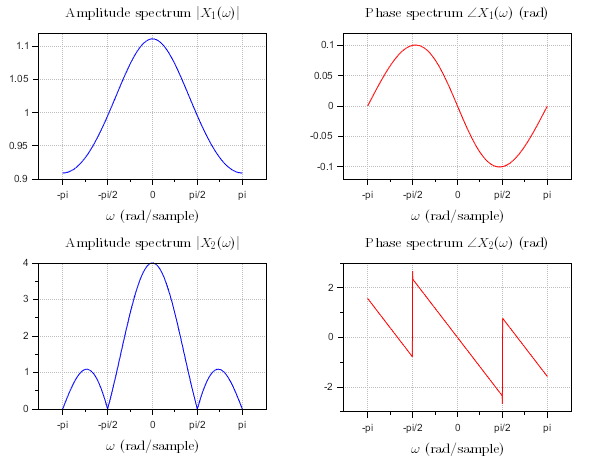
\includegraphics[width=0.9\linewidth]{ex6.3_0.png}
    \caption{Phổ biên độ (trái) và phổ pha (phải) của $x_1(n)$ (trên) và $x_2(n)$ (dưới)}
    \label{fig:ex63}
\end{figure}

Console cho thấy $X_1$ tính bằng tổng số và bằng công thức chỉ lệch $6.7 \times 10^{-16}$; các giá trị $|X_1(0)| = 1.1111$, $|X_1(\pi)| = 0.9091$, $|X_2(0)| = 4$ và $|X_2(\pi/2)| = |X_2(\pi)| \approx 0$ đúng như tính tay. Trên Hình~\ref{fig:ex63}, cả hai phổ biên độ đều là hàm chẵn và phổ pha là hàm lẻ theo $\omega$, đúng với tính chất của tín hiệu thực. $|X_1(\omega)|$ biến thiên rất ít (từ $0.91$ đến $1.11$), còn $|X_2(\omega)|$ có dạng một búp chính ở $\omega = 0$ và các búp phụ nhỏ hơn, đặc trưng của xung chữ nhật. Pha của $x_2$ tuyến tính và nhảy $\pi$ tại $\omega = \pm\frac{\pi}{2}$, nơi biên độ bằng 0.

% =====================================================================
\subsection{Bài tập 4 -- Đáp ứng tần số của hệ LTI}
\begin{mdframed}[style=exbox]
\noindent\textbf{Bài tập 4.} Cho hệ LTI mô tả bởi phương trình sai phân
\[
    y(n) + 0.1y(n-1) + 0.2y(n-2) = x(n).
\]
Xác định biến đổi Fourier của đáp ứng xung $h(n)$, sau đó vẽ phổ biên độ và phổ pha.
\end{mdframed}

\noindent\textbf{1. Cơ sở lý thuyết và tính toán:}

Lấy biến đổi Fourier hai vế, dùng tính chất dịch thời gian $x(n - k) \fpair e^{-j\omega k}X(\omega)$:
\begin{equation}
    H(\omega) = \frac{Y(\omega)}{X(\omega)} = \frac{1}{1 + 0.1e^{-j\omega} + 0.2e^{-j2\omega}}.
\end{equation}
Biến đổi Fourier này tồn tại vì hệ ổn định: hai cực là nghiệm của $z^2 + 0.1z + 0.2 = 0$, tức $z = -0.05 \pm j0.4444$, có $|p| = \sqrt{0.2} \approx 0.447 < 1$. Một vài giá trị đặc biệt:
\[
    H(0) = \frac{1}{1 + 0.1 + 0.2} = 0.7692, \qquad H(\pi) = \frac{1}{1 - 0.1 + 0.2} = 0.9091.
\]
Từ cặp cực phức $re^{\pm j\theta}$ với $r = \sqrt{0.2}$, $\theta \approx 96.42^\circ$, đáp ứng xung có dạng
\[
    h(n) = \left(\sqrt{0.2}\right)^n \left[\cos(n\theta) - 0.1125\sin(n\theta)\right] u(n),
\]
với các giá trị đầu $1, -0.1, -0.19, 0.039, 0.0341, \dots$

\noindent\textbf{2. Mã nguồn thực thi trên Scilab:}
\lstinputlisting[language=Scilab, style=scilabstyle]{../scilab_src/Ex_6.4.sci}

\noindent\textbf{3. Kết quả mô phỏng và nhận xét:}
\begin{lstlisting}[style=consolestyle]
--> exec('Ex_6.4.sci', -1)
   1.  -0.1  -0.19   0.039   0.0341  -0.01121
  "h(0..5) ="
   6.959D-15
  "sai lech lon nhat giua H tinh so va cong thuc ="
   0.7692308
  "|H(0)| ="
   0.9090909
  "|H(pi)| ="
\end{lstlisting}

\begin{figure}[H]
    \centering
    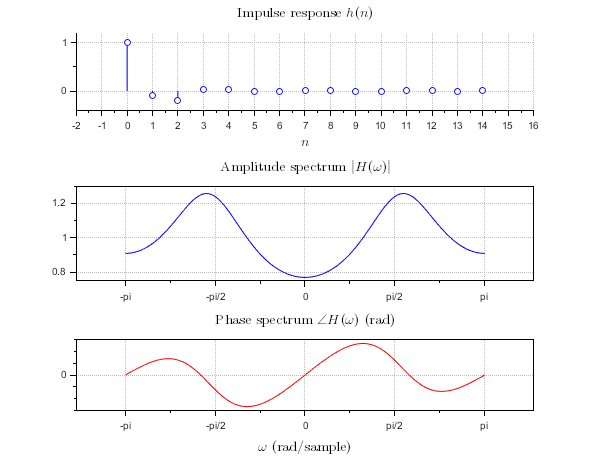
\includegraphics[width=0.85\linewidth]{ex6.4_0.png}
    \caption{Đáp ứng xung $h(n)$, phổ biên độ $|H(\omega)|$ và phổ pha $\angle H(\omega)$}
    \label{fig:ex64}
\end{figure}

$h(n)$ tính bằng hàm \texttt{filter} trùng với các giá trị đầu từ công thức, và DTFT của $h(n)$ lệch với công thức $H(\omega)$ chỉ $7 \times 10^{-15}$. Trên Hình~\ref{fig:ex64}, $h(n)$ dao động và tắt rất nhanh vì $|p| \approx 0.447$. Phổ biên độ nhỏ nhất tại $\omega = 0$ ($0.769$) và đạt đỉnh quanh $\omega \approx \pm 0.54\pi$, gần với góc của cặp cực $\theta \approx 96^\circ \approx 0.54\pi$: đúng như lý thuyết, biên độ tăng ở những tần số mà điểm $e^{j\omega}$ trên đường tròn đơn vị nằm gần cực. Do cực không quá gần đường tròn đơn vị nên đỉnh chỉ cao khoảng $1.26$, phổ khá thoải. Phổ pha là hàm lẻ, dao động trong khoảng nhỏ quanh 0.

% =====================================================================
\subsection{Bài tập 5 -- Tìm ngõ ra bằng biến đổi Fourier}
\begin{mdframed}[style=exbox]
\noindent\textbf{Bài tập 5.} Cho hệ LTI có $h(n) = \delta(n) + \delta(n-1)$. Dùng biến đổi Fourier để xác định ngõ ra $y(n)$ khi ngõ vào $x(n) = 0.5^n u(n)$. Sau đó dùng Scilab vẽ phổ biên độ và phổ pha.
\end{mdframed}

\noindent\textbf{1. Cơ sở lý thuyết và tính toán:}

Biến đổi Fourier của hệ và của tín hiệu vào:
\[
    H(\omega) = 1 + e^{-j\omega}, \qquad X(\omega) = \frac{1}{1 - 0.5e^{-j\omega}}.
\]
Theo tính chất tích chập, $y(n) = x(n) * h(n) \fpair Y(\omega) = H(\omega)X(\omega)$:
\[
    Y(\omega) = \frac{1 + e^{-j\omega}}{1 - 0.5e^{-j\omega}}.
\]
Chia đa thức theo $e^{-j\omega}$: $1 + e^{-j\omega} = -2\left(1 - 0.5e^{-j\omega}\right) + 3$, nên
\[
    Y(\omega) = -2 + \frac{3}{1 - 0.5e^{-j\omega}}.
\]
Lấy biến đổi ngược từng thành phần ($1 \fpair \delta(n)$ và $\frac{1}{1 - 0.5e^{-j\omega}} \fpair 0.5^n u(n)$):
\begin{equation}
    y(n) = 3\,(0.5)^n u(n) - 2\delta(n) = \{\underset{\uparrow}{1}, 1.5, 0.75, 0.375, \dots\}.
\end{equation}
\textbf{Kiểm tra} bằng tích chập trực tiếp: $y(n) = x(n) + x(n-1)$, nên $y(0) = 1$, $y(1) = 0.5 + 1 = 1.5$, $y(2) = 0.25 + 0.5 = 0.75$, khớp.

Về phổ: $|H(\omega)| = 2\left|\cos\frac{\omega}{2}\right|$ và $\angle H(\omega) = -\frac{\omega}{2}$, là bộ lọc thông thấp có $H(\pm\pi) = 0$. $|X(\omega)| = \frac{1}{\sqrt{1.25 - \cos\omega}}$, lớn nhất bằng 2 tại $\omega = 0$. Do đó $|Y(\omega)| = |H(\omega)||X(\omega)|$ bằng 4 tại $\omega = 0$ và bằng 0 tại $\omega = \pm\pi$, còn $\angle Y(\omega) = \angle H(\omega) + \angle X(\omega)$.

\noindent\textbf{2. Mã nguồn thực thi trên Scilab:}
\lstinputlisting[language=Scilab, style=scilabstyle]{../scilab_src/Ex_6.5.sci}

\noindent\textbf{3. Kết quả mô phỏng và nhận xét:}
\begin{lstlisting}[style=consolestyle]
--> exec('Ex_6.5.sci', -1)
   1.   1.5   0.75   0.375   0.1875   0.09375
  "y(0..5) tinh bang tich chap ="
   1.   1.5   0.75   0.375   0.1875   0.09375
  "y(0..5) tinh tu bien doi Fourier ="
   0.
  "sai lech lon nhat ="
   5.457D-12
  "sai lech giua Y(w) = H.X va DTFT cua y(n) ="
\end{lstlisting}

\begin{figure}[H]
    \centering
    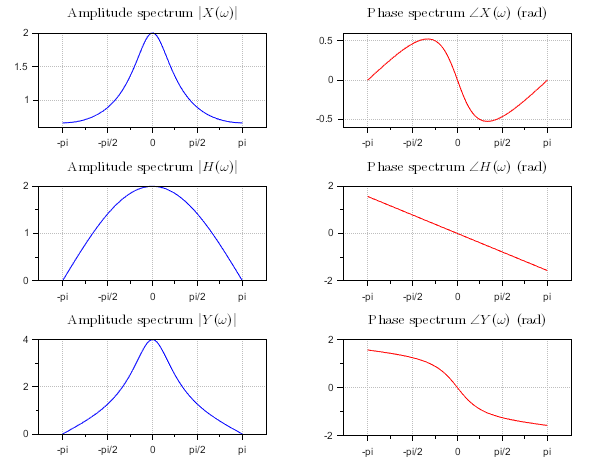
\includegraphics[width=0.85\linewidth]{ex6.5_0.png}
    \caption{Phổ biên độ (trái) và phổ pha (phải) của $X(\omega)$, $H(\omega)$ và $Y(\omega)$}
    \label{fig:ex65spec}
\end{figure}

\begin{figure}[H]
    \centering
    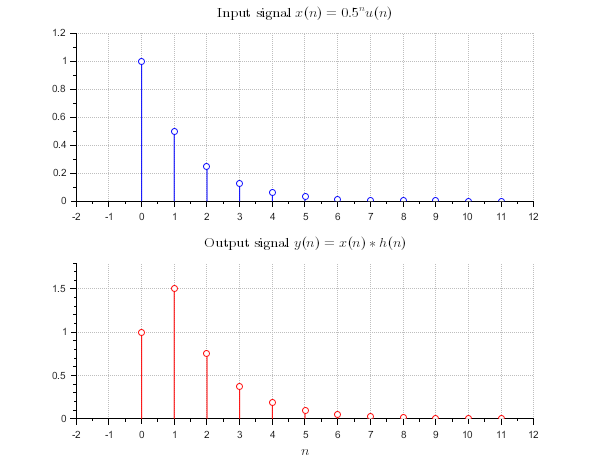
\includegraphics[width=0.75\linewidth]{ex6.5_1.png}
    \caption{Tín hiệu vào $x(n) = 0.5^n u(n)$ và ngõ ra $y(n)$}
    \label{fig:ex65time}
\end{figure}

Ngõ ra tính bằng tích chập và tính từ biến đổi Fourier trùng nhau hoàn toàn (sai lệch bằng 0). Sai lệch $5 \times 10^{-12}$ giữa $Y(\omega) = H(\omega)X(\omega)$ và DTFT của $y(n)$ chỉ do script cắt $y(n)$ còn 40 mẫu ($0.5^{40} \approx 10^{-12}$). Trên Hình~\ref{fig:ex65spec}, $|H(\omega)|$ giảm dần về 0 tại $\omega = \pm\pi$ (lọc thông thấp), pha của $H$ là đường thẳng $-\frac{\omega}{2}$; nhân với $|X(\omega)|$ cũng tập trung ở tần số thấp nên $|Y(\omega)|$ có đỉnh bằng 4 tại $\omega = 0$ và bằng 0 tại $\omega = \pm\pi$. Trong miền thời gian (Hình~\ref{fig:ex65time}), $y(n)$ là tổng của $x(n)$ và bản trễ một mẫu của nó, nên $y(1) = 1.5$ lớn hơn $y(0)$, sau đó giảm theo $0.5^n$.

\section{Bàn Luận}
Qua bài thực hành, em thấy biến đổi Fourier của tín hiệu rời rạc chính là biến đổi Z trên đường tròn đơn vị, nên các kỹ năng ở Lab 4--5 (tổng cấp số nhân, tính chất dịch, khai triển phân thức) dùng lại được gần như nguyên vẹn. Các phổ vẽ trên Scilab đều đúng với lý thuyết: phổ biên độ của tín hiệu thực là hàm chẵn, phổ pha là hàm lẻ, xung chữ nhật cho phổ dạng sinc với pha tuyến tính, và đỉnh của $|H(\omega)|$ xuất hiện gần góc của các cực. Bài 5 cho thấy tìm ngõ ra bằng $Y(\omega) = H(\omega)X(\omega)$ gọn hơn tính tổng tích chập. Hai điểm em cần lưu ý là: biến đổi Fourier chỉ tồn tại khi tín hiệu khả tổng tuyệt đối (hoặc hệ ổn định), nên tín hiệu $x_5(n)$ ở Bài 2 phải hiểu là nhân quả; và khi xuất hình bằng Scilab ở chế độ chạy tự động, cần đợi hình vẽ xong rồi mới lưu, nếu không hình có thể bị thiếu.

\section{Tài Liệu Tham Khảo}
Đường link GitHub chứa mã nguồn thực hành source code SciLab: \url{https://github.com/qanetta/DigitalSignalProcessing-Lab.git}

\end{document}
